\documentclass[12pt,aspectratio=169]{beamer}
\usetheme{default}
\usecolortheme{dolphin}
\usefonttheme{structurebold}

\title{ShellScript 01}
\author{@aoirint}
\date{2020/04/16}
%\institute{}

\begin{document}

% 01
\frame{\maketitle}

% 02
\begin{frame}{テキスト}

  \begin{minipage}{0.58\textwidth}
    \begin{itemize}
      \item 新しいシェルプログラミングの教科書
      \begin{itemize}
        \item 著・三宅英明
        \item 刊・SB Creative
      \end{itemize}
    \end{itemize}
  \end{minipage}
  \hfill
  \begin{minipage}{0.38\textwidth}
    \vspace{-4\baselineskip}
    \begin{center}
      
\includegraphics[width=5cm,bb=0 0 467 596]{./images/shellbook.jpg}
    \end{center}
  \end{minipage}

  \begin{itemize}
    \item 書影
    \begin{itemize}
      \item { \small \url{https://www.sbcr.jp/product/4797393101/} }
    \end{itemize}
  \end{itemize}

\end{frame}

\begin{frame}{GUI 1/2}
  \centering {
    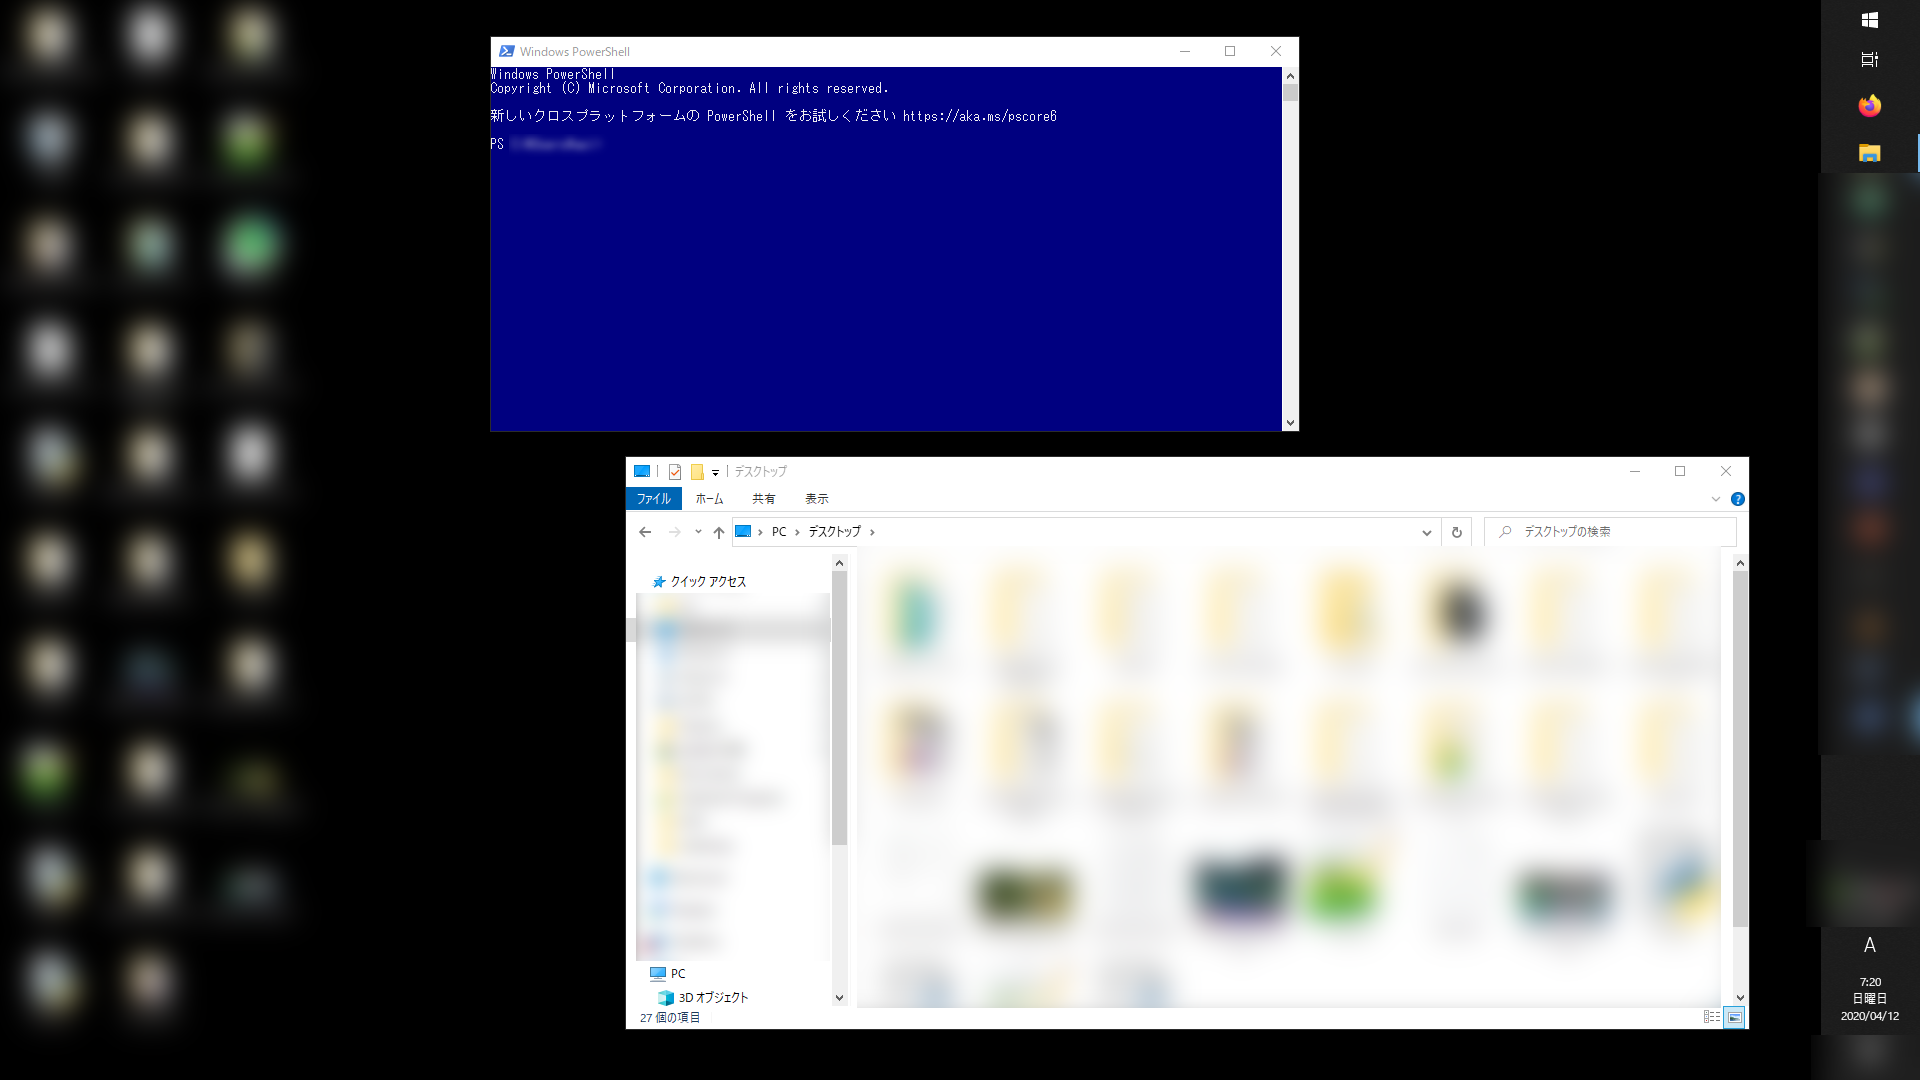
\includegraphics[width=12cm,bb=0 0 1920 1080]{./images/windows-explorer.png}

    Windows Explorer
  }
\end{frame}

\begin{frame}{GUI 2/2}
  \centering {
    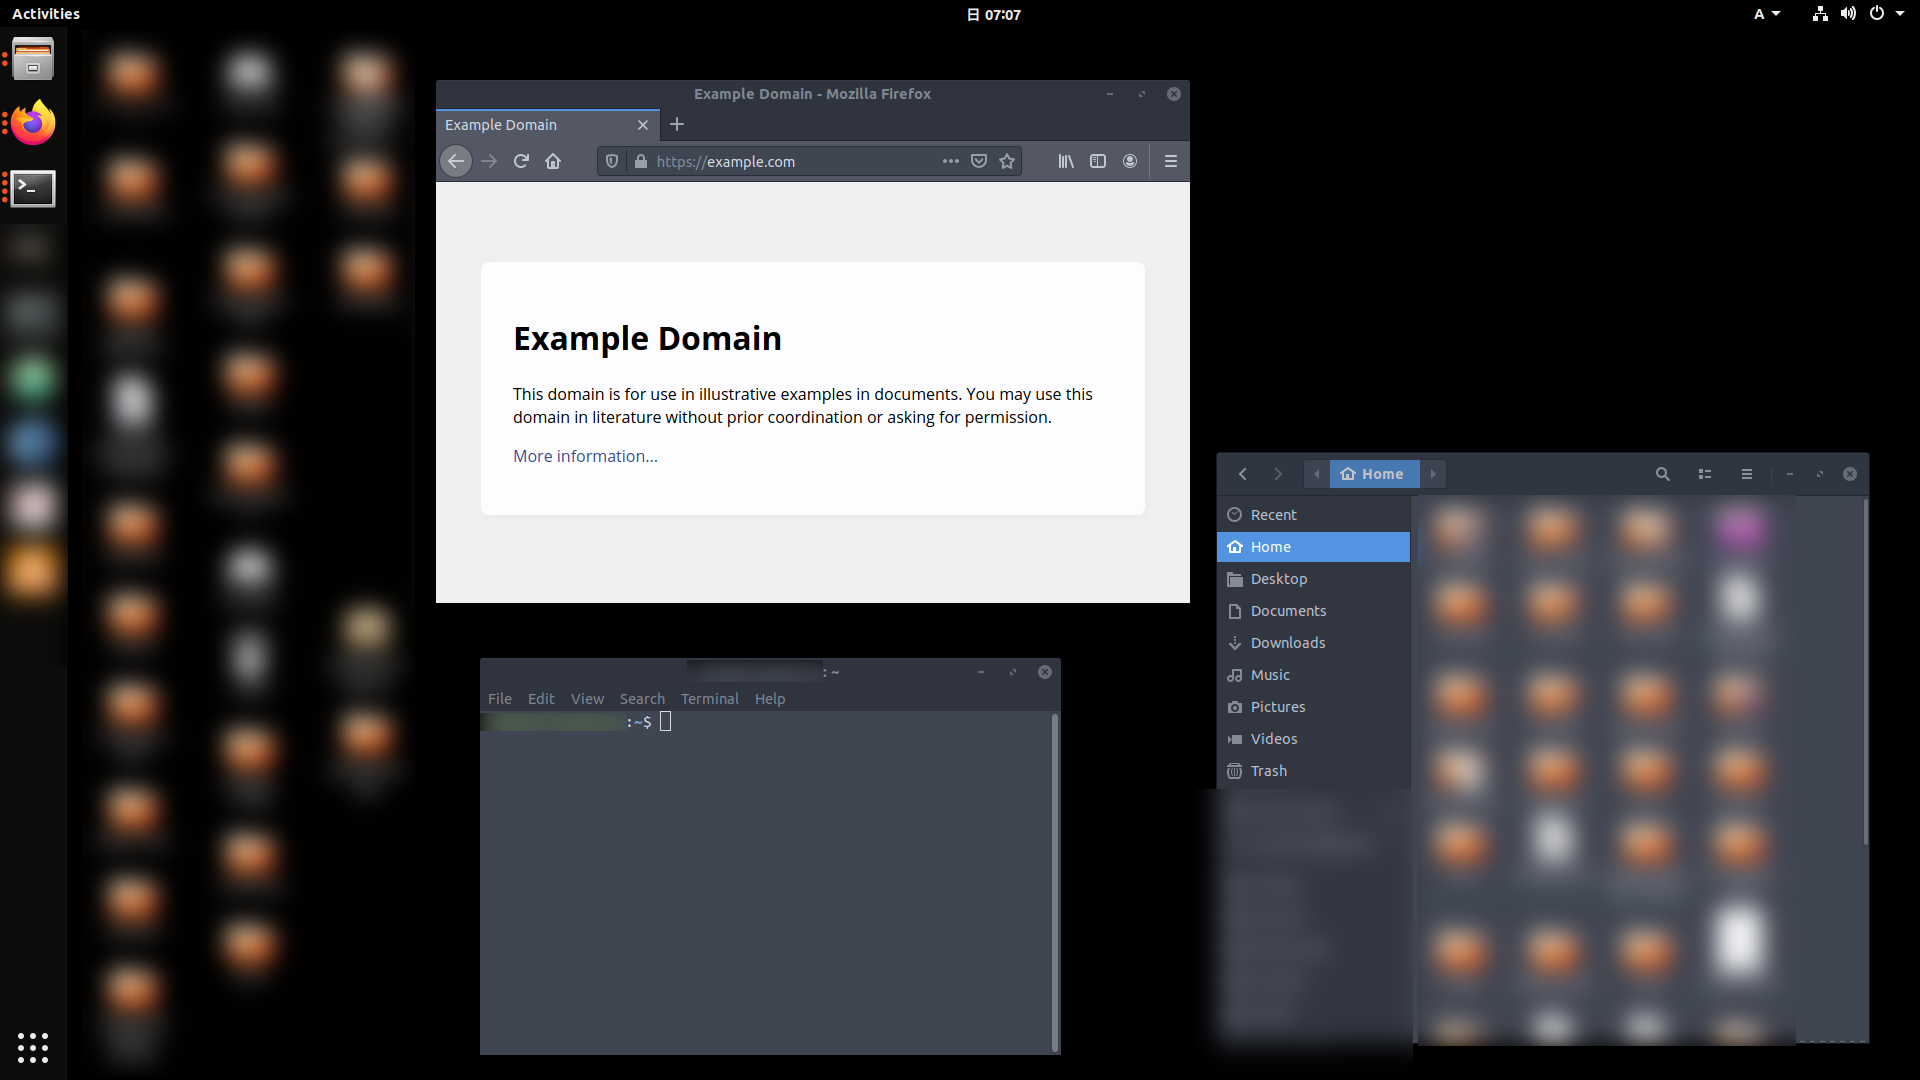
\includegraphics[width=12cm,bb=0 0 1920 1080]{./images/gnome-desktop.png}

    Ubuntu Gnome Desktop
  }
\end{frame}

\begin{frame}{CLI}

  \begin{minipage}{0.3\textwidth}
    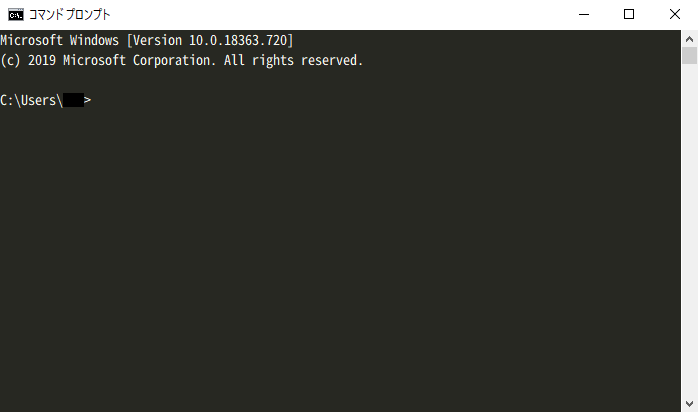
\includegraphics[width=1.2\linewidth,bb=0 0 698 412]{./images/cmd.png}
    コマンドプロンプト(Windows)

    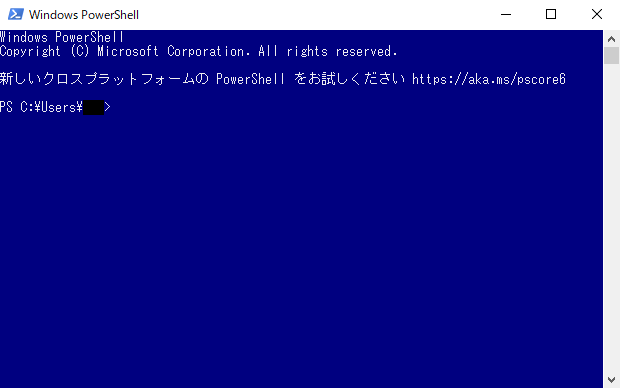
\includegraphics[width=1.2\linewidth,bb=0 0 620 388]{./images/powershell.png}
    Powershell(Windows)
  \end{minipage}
  \hfill
  \begin{minipage}{0.3\textwidth}
    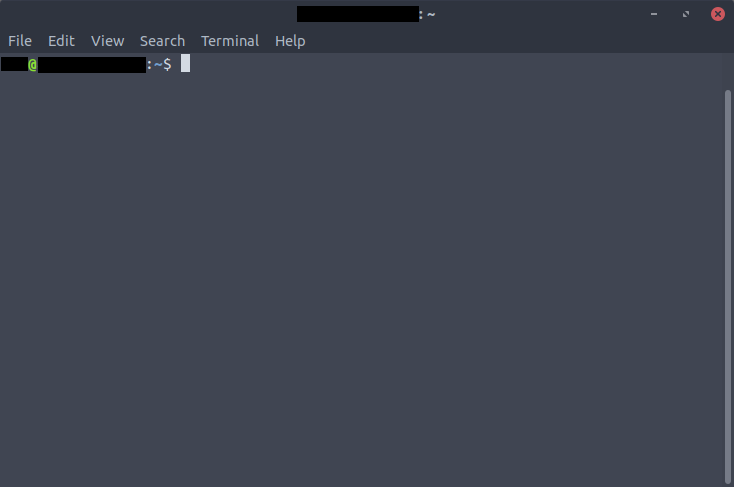
\includegraphics[width=\linewidth,bb=0 0 734 487]{./images/ubuntu-gnome.png}
    \begin{flushleft} \small Terminal(Ubuntu,Gnome) \end{flushleft}
    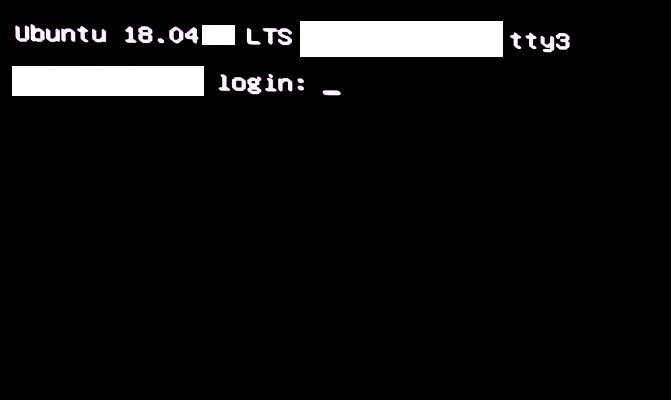
\includegraphics[width=\linewidth,bb=0 0 734 487]{./images/ubuntu-cli.jpg}
    CLI(Ubuntu)
  \end{minipage}
  \hfill
  \begin{minipage}{0.3\textwidth}
    \vspace{-5\baselineskip}
    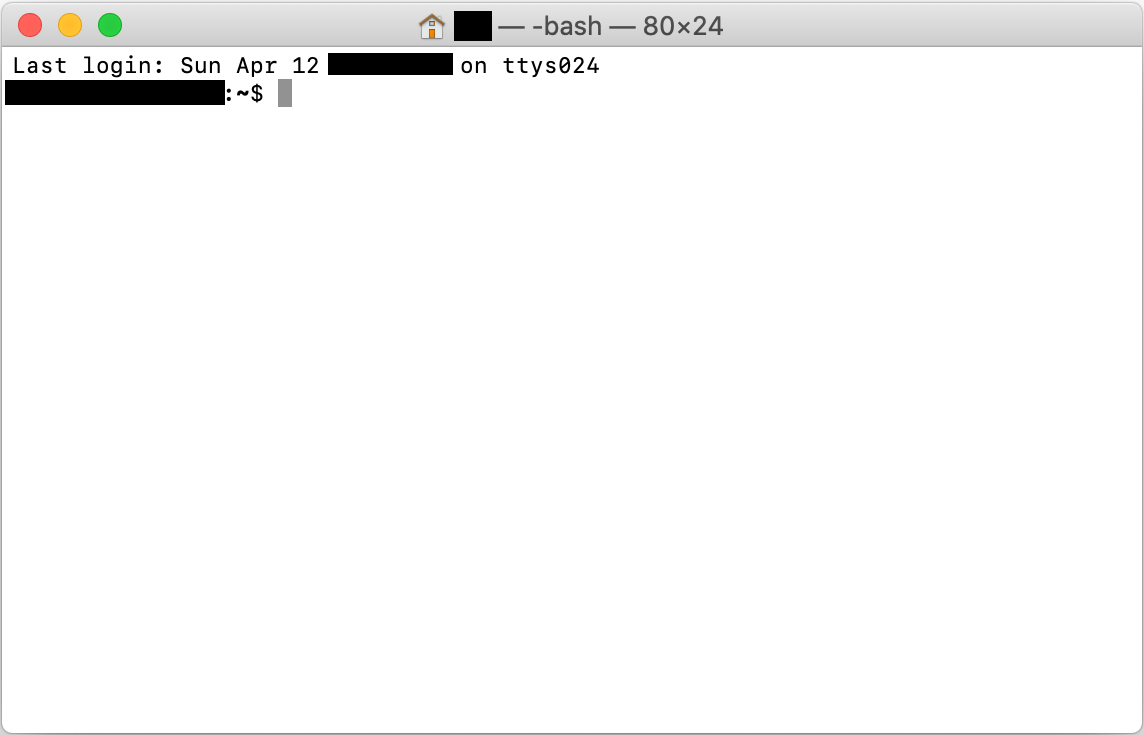
\includegraphics[width=2.0\linewidth,bb=0 0 1144 735]{./images/mac-basic.png}
    Terminal(macOS)
  \end{minipage}

\end{frame}

\begin{frame}{シェルとは}
  \centering
  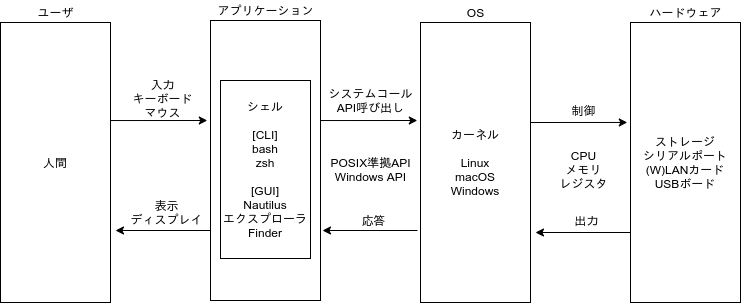
\includegraphics[width=12cm,bb=0 0 741 281]{./images/shell.png}

\end{frame}


\begin{frame}{Tips: Windows エクスプローラにコンテキストメニューを追加する}

\end{frame}

\begin{frame}{以上です}
てすと

\end{frame}


\end{document}
